\documentclass[12 pt]{beamer}
\usetheme[
  bullet=circle,		% Other option: square
  bigpagenumber,		% circled page number on lower right
  topline=true,			% colored bar at the top of the frame 
  shadow=false,			% Shading for beamer blocks
  watermark=BG_lower,	% png file for the watermark
]{Flip}


\newcommand{\titleimage}{title}			% Custom title 
\newcommand{\tanedo}{tanedolight}		% Custom author name
\newcommand{\CMSSMDM}{CMSSMDMlight.png}	% light background plot


%%%%%%%%%%
% FONTS %
%%%%%%%%%%

\usepackage[T1]{fontenc}
%\usepackage{lmodern}		
%\usepackage{sfmath}		% Sans Serif Math, off by default

%% Protects fonts from Beamer screwing with them
%% http://tex.stackexchange.com/questions/10488/force-computer-modern-in-math-mode
\usefonttheme{professionalfonts}


\usepackage[no-math]{fontspec}		

%\defaultfontfeatures{Mapping=tex-text}	% This seems to be important for mapping glyphs properly

\usepackage{amsmath}
%\usepackage{amsfonts}
%\usepackage{amssymb}
\usepackage{mathspec}
\usepackage{graphicx}
%\usepackage{mathrsfs} 			% For Weinberg-esque letters
\usepackage{cancel}				% For "SUSY-breaking" symbol
\usepackage{slashed}            % for slashed characters in math mode
%\usepackage{bbm}                % for \mathbbm{1} (unit matrix)
\usepackage{amsthm}				% For theorem environment
\usepackage{multirow}			% For multi row cells in table
\usepackage{arydshln} 			% For dashed lines in arrays and tables
usepackage{tikzfeynman}		% For Feynman diagrams
% \usepackage{subfig}           % for sub figures
% \usepackage{young}			% For Young Tableaux
% \usepackage{xspace}			% For spacing after commands
% \usepackage{wrapfig}			% for Text wrap around figures
% \usepackage{framed}

\usepackage{setspace}

\setsansfont{calibri}[ 
Extension = .ttf,
UprightFont = *,
BoldFont = *b,
ItalicFont = *i,
Scale = 1
]

\setmathfont(Digits,Latin,Greek){SitkaI.ttc}

\graphicspath{{images/}}	% Put all images in this directory. Avoids clutter.


\usetikzlibrary{backgrounds}
\usetikzlibrary{mindmap,trees}	% For mind map
\usetikzlibrary{arrows,positioning,calc}
\usetikzlibrary{shapes}
% http://www.texample.net/tikz/examples/computer-science-mindmap/


% SOME COMMANDS THAT I FIND HANDY
% \renewcommand{\tilde}{\widetilde} % dinky tildes look silly, dosn't work with fontspec
\newcommand{\comment}[1]{\textcolor{comment}{\footnotesize{#1}\normalsize}} % comment mild
\newcommand{\Comment}[1]{\textcolor{Comment}{\footnotesize{#1}\normalsize}} % comment bold
\newcommand{\COMMENT}[1]{\textcolor{COMMENT}{\footnotesize{#1}\normalsize}} % comment crazy bold
\newcommand{\Alert}[1]{\textcolor{Alert}{#1}} % louder alert
\newcommand{\ALERT}[1]{\textcolor{ALERT}{#1}} % loudest alert
%% "\alert" is already a beamer pre-defined



\author{}
\title{Informatikai Rendszerek Biztonságtechnikája}
\institute{}
\date{}



\begin{document}

%% To use external nodes; http://www.texample.net/tikz/examples/beamer-arrows/
\tikzstyle{every picture}+=[remember picture]

{
  \setbeamertemplate{sidebar right}{\llap{
\includegraphics[width=\paperwidth,height=\paperheight]{backgnd}}}

  \begin{frame}[c]
    \begin{center}
      % \includegraphics[width=7cm]{WarpedPenguinsReturn}

      \Large
      \textbf{Információs rendszerek}

      \textbf{biztonságtechnikája}

      \qquad

      Kriptográfia

      Szimmetrikus kódú algoritmusok

      \qquad

      \textit{Vakulya Gergely}



      %\begin{tikzpicture}%[show background grid] %% Use grid for positioning, then turn off
      %	\node[inner sep=0pt,above right] (title) 
      %		{ \includegraphics[width=7cm]{\titleimage} };
      %	% \node (title) at (1.5,1.5) {};
      %\end{tikzpicture}
      %\quad

      % \includegraphics[width=7cm]{\titleimage} 

      %\vspace{1em}
      %\footnotesize\textcolor{gray}{Journal of Cool Beans
      %\texttt{[arXiv:1234.5678]}}
      %\vspace{.5em}

      %\includegraphics[height=1.5cm]{\tanedo} \quad
      % {\fontspec{Zapfino} Flip Tanedo} \quad
      % \includegraphics[height=1cm]{FlipSansSerif} \quad
      %\includegraphics[height=1.5cm]{CUasym}\\
      % \footnotesize\textcolor{gray}{In collaboration with} Csaba Cs\'aki\textcolor{gray}{,} Yuval Grossman\textcolor{gray}{, and} Yuhsin Tsai\normalsize\\
      %	\footnotesize\textcolor{gray}{In collaboration with 
      %		D. Grayson, J. Todd, T. Drake, S. Brown, D. Wayne}\normalsize\\
      %	\textcolor{normal text.fg!50!Comment}{\textit{Gotham University}, \today}
      % \textcolor{Comment}{ \;($\pi$ day)}\\
      % \Comment{4 February 2011}
    \end{center}
  \end{frame}
  }

  %------------------------------------------------

\begin{frame}{A kriprográfia négy célja}

  \begin{block}{Titkosság (secrecy, confidentality)}
    Annak biztosítása, hogy az üzenetet harmadik fél \textbf{ne tudja elolvasni}.
  \end{block}

  \begin{block}{Hitelesség (authentication)}
    Annak bizonyíthatósága, hogy az üzenet valóban a \textbf{feladótól származik}.
  \end{block}

  \begin{block}{Letagadhatatlanság (nonrepudiation)}
    Annak bizonyíthatósága, hogy az üzenetet a \textbf{feladó valóban elküldte}.
  \end{block}

  \begin{block}{Sértetlenség (integrity)}
    Annak biztosítása, hogy az üzenetet harmadik személy \textbf{ne tudja megváltoztatni}.
  \end{block}
  
\end{frame}

%------------------------------------------------

\begin{frame}{A kriptográfia modellje}

  \begin{block}{Jelölések}
    \begin{itemize}
      \item{Nyílt szöveg (plaintext), $P$}
      \item{Kulcs (key), $K$}
      \item{Titkosított szöveg (cyphertext), $C$}
    \end{itemize}
  \end{block}

  \[C = E_K(P)\]

  \[P = D_K(C)\]

  \[D_K(E_K(P)) = P\]
  
  \begin{block}{Kerchoff elve}
    \textbf{Minden algoritmusnak nyilvánosnak kell lennie; csak a kulcsok titkosak (1883)}
  \end{block}

\end{frame}
    
%------------------------------------------------

\begin{frame}{Kriptoanalízis}
  \begin{block}{Csak titkosított szöveg alapú támadás}
    A kódtöréshez csak egy, vagy több titkosított szöveget ismerünk. A legnehezebb szituáció.
  \end{block}

  \begin{block}{Ismert nyílt szöveg alapú támadás}
    Nyílt szöveg - titkosított szöveg párokat ismerünk. Talán ez a leggyakoribb eset.
  \end{block}

  \begin{block}{Választott nyílt szöveg alapú támadás}
    Lehetőségünk van tetszőleges nyílt szöveget titkosítani (tehát a nyílt szövegekhez előállítani azok titkosított szöveg párját), de magát a kulcsot nem ismerjük. Ez az eset nyilvános kulcsú algoritmusok, illetve ,,blackbox'' titkosítók esetében fordul elő.
  \end{block}
\end{frame}

%------------------------------------------------

\begin{frame}{Az ismeretlenség biztonsága (security by obscurity)}
  A rendszer (nem feltétlenül titkosítási eljárás) működésével kapcsolatban bizonyos gyengeségeket szándékosan nem hoznak nyilvánosságra azt remélve, hogy azokat nem fedezik fel / használják ki. Napellenzőbe ,,rejtett'' forgalmi engedély, lábtörlő alá ,,rejtett'' kulcs esete.

  \begin{itemize}
    \item{Zárt forráskódú firmware-ek.}
    \item{A fájlrendszer mélyére ,,jól elrejtett'' fájlokban tárolt érzékeny adatok.}
    \item{Beépített kiskapuk (például pótjelszavak).}
  \end{itemize}

  \begin{alertblock}{}
    \centering Rossz gyakorlat. Kerülendő!
  \end{alertblock}

\end{frame}

%------------------------------------------------

\begin{frame}{A feltörhetetlen kód (one-time pad)}
  \begin{columns}
    \begin{column}{0.63\textwidth}
      \begin{block}{A kizáró vagy (XOR) művelet}
        \begin{itemize}
          \item{$K \oplus K = 0$}
          \item{$C = P \oplus K$}
          \item{$P = C \oplus K = P \oplus K \oplus K$}
          \item{Egy kulcs csak egyszer használható fel!}
        \end{itemize}
      \end{block}
    \end{column}
    \begin{column}{0.35\textwidth}
      \begin{center}
        \begin{tabular}{ |c|c||c| } 
         \hline
         $A$ & $B$ & $A \oplus B$ \\
          \hline
         0 & 0 & 0 \\ 
          \hline
         0 & 1 & 1 \\ 
          \hline
         1 & 0 & 1 \\ 
          \hline
         1 & 1 & 0 \\ 
          \hline
        \end{tabular}
      \end{center}
    \end{column}
  \end{columns}
  \begin{block}{A titkosítás menete}
    \begin{itemize}
      \item{Alice és Bob megállapodnak egy közös kulcsban.}
      \item{A kódolás akkor működőképes, ha a kulcs véletlenszerű bitekből áll és legalább akkora, mint a kódolandó adat.}
      \item{Például Alice generál egy DVD-nyi véletlenszerű bitet és a lemezt eljuttatja Bobnak.}
      \item{Ezt követően bármelyikük titkos kommunikációt tud folytatni a másikkal a kulcs (a DVD) méretéig bezárólag.}
    \end{itemize}
  \end{block}
\end{frame}

%------------------------------------------------

\begin{frame}{A feltörhetetlen kód (one-time pad)}
  \begin{columns}
    \begin{column}{0.55\textwidth}
      \begin{block}{Hátrányok}
        \begin{itemize}
          \item{A kulcs elkészítése problematikus.}
            \begin{itemize}
              \item{A számítógép általában pszeudorandom szekvenciákat tud gyorsan generálni.}
              \item{Ténylegesen véletlen számok előállítása nehéz / lassú.}
            \end{itemize}
          \item{A kulcs megosztása, tárolása problematikus.}
            \begin{itemize}
              \item{Elzárva kell tartani.}
              \item{Könnyen lemásolhatják.}
            \end{itemize}
        \end{itemize}
      \end{block}
    \end{column}
    \begin{column}{0.44\textwidth}
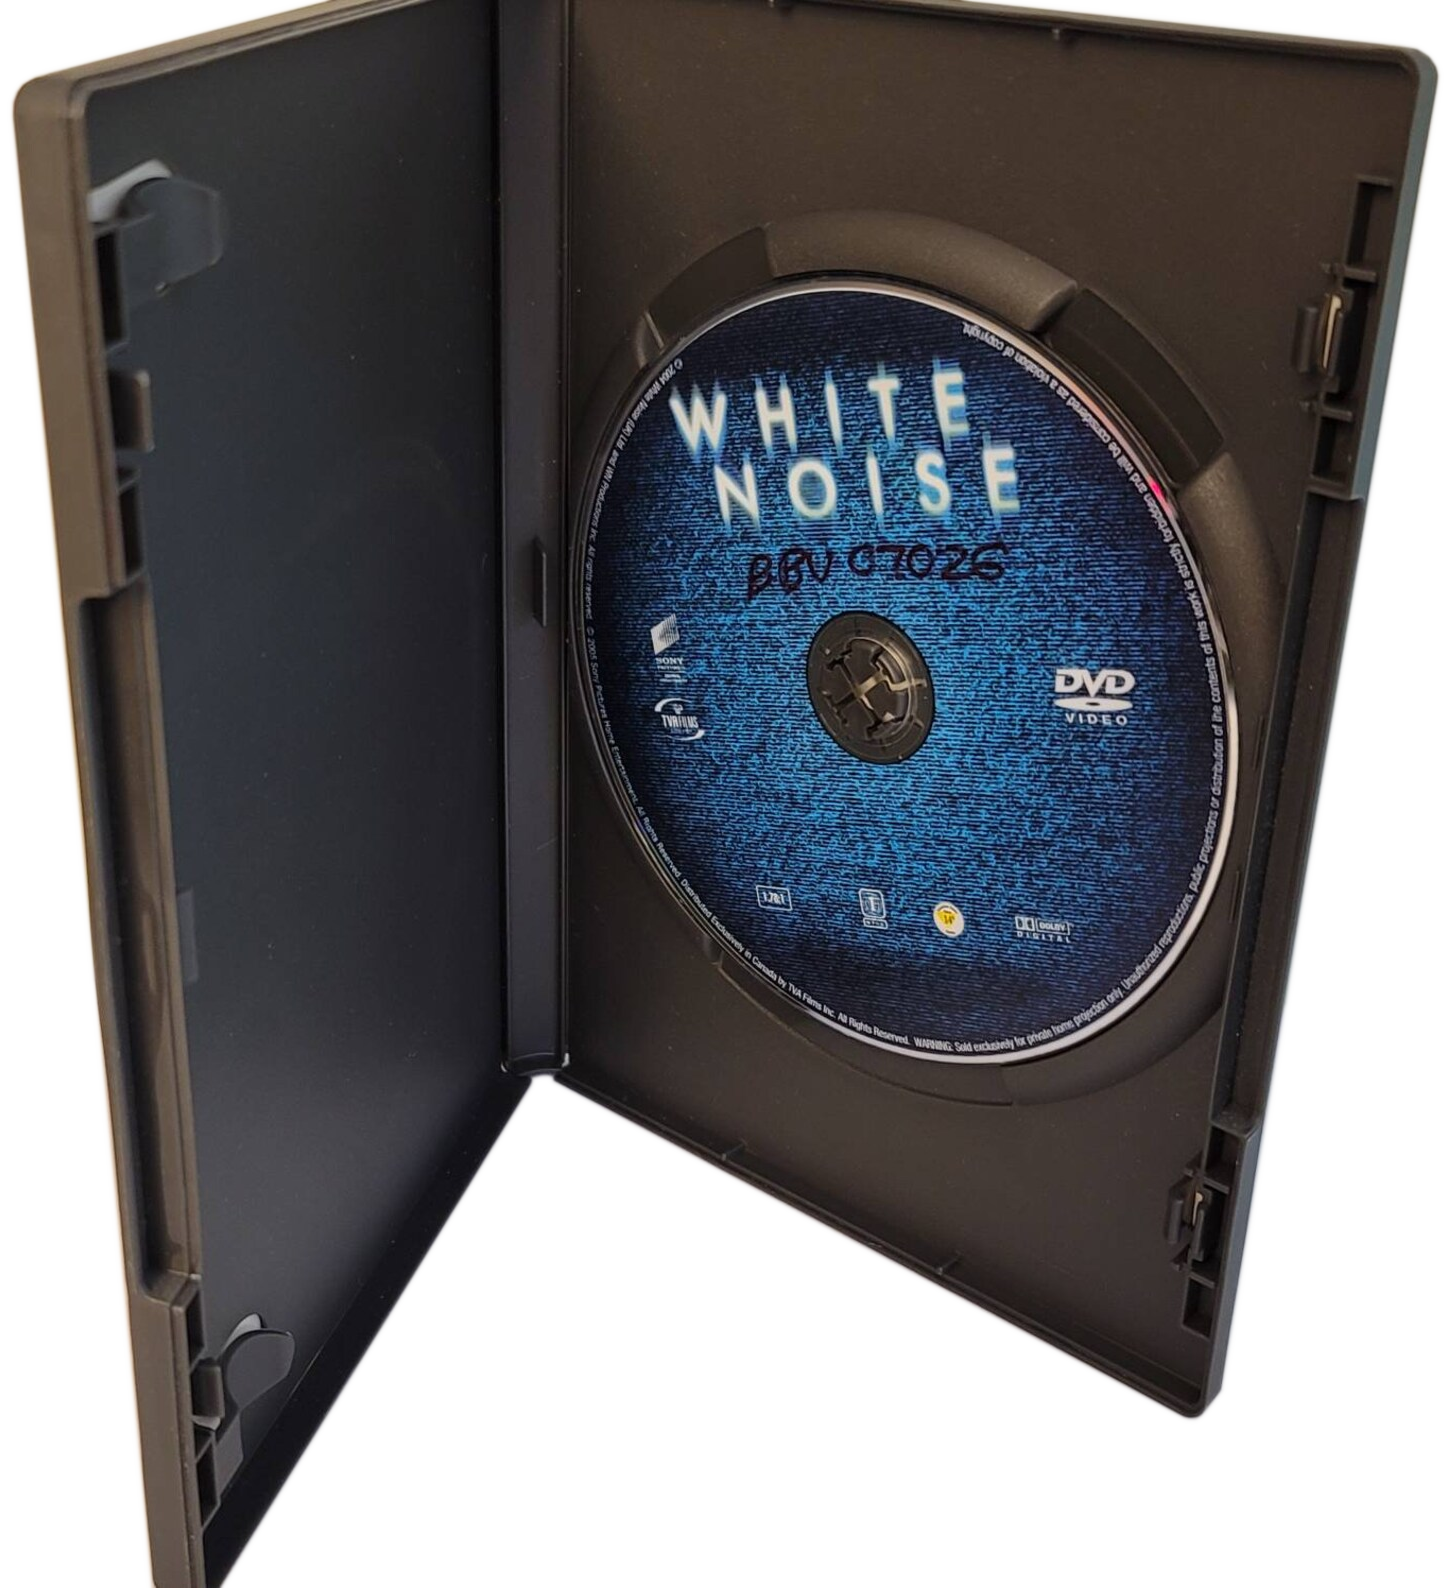
\includegraphics[width=\textwidth]{whitenoise}
    \end{column}
  \end{columns}
\end{frame}

%\begin{frame}{Szimmetrikus kulcsú titkosítások}
%  S doboz
%
%  P doboz
%
%
%\usetikzlibrary{arrows,positioning,calc}
%    \begin{tikzpicture}[>=latex]
%        \node[draw,inner sep=1.5cm] (a) {$A$};
%        \node at (-7,0) (pk) {pk};
%            \draw[->] (pk) -- (a);
%        \node[below=.2 of pk] (ms) {$m^*,s^*$};
%            \draw[<-] (ms) --+ (5.35,0) node[midway,align=center,below,text width=4cm] {Win if \textsf{\textcolor{blue}{Verify$_{pk}$}$(s^*,m^*)=\mathtt{valid}$ and $m^*\not\in\textcolor{red}{\mathcal{L}}$}};
%            \node (n) at ([yshift=-.5cm,xshift=.5cm]a) {$m\in\mathbb{P}$};
%            \draw[->] ($(n)+(1.15,0)$) --+ (2.8,0) node[midway,above] {$\mathcal{O}_{\textsf{Sig}_{\mathfrak{s\!k}}}$};
%                \node[right] at ($(n)+(3.85,0)$) {$\textcolor{red}{\mathcal{L}}\leftarrow\textcolor{red}{\mathcal{L}}\cup\{m\}$};
%            \draw[->] (4.4,-1) --+ (-2.75,0);
%                \node[yshift=-.5cm,right] at ($(n)+(3.85,0)$) {$t\leftarrow\textcolor{red}{\textsf{Sig}_{\textcolor{blue}{\mathfrak{sk}}}}(m)$};
%                \node[xshift=1.5cm,above=.5 of pk] {$(\textcolor{blue}{\mathfrak{pk}},\textcolor{red}{\mathfrak{sk}})\leftarrow\mathrm{KeyGen()}$};
%                \node[xshift=11cm,above=.5 of pk] {$\textcolor{red}{\mathcal{L}}\leftarrow\emptyset$};
%    \end{tikzpicture}
%
%\end{frame}

\begin{frame}{Szimmetrikus kulcsú titkosítások}
  \begin{itemize}
    \item{A szimmetrikus kulcsú algoritmusok mind a kódoláshoz, mind a dekódoláshoz \textbf{ugyanazt a kulcsot} használják.}
    \item{A blokk kódolók $n$ bites blokkokra bontják a bemenetet és a kódolást / dekódolást ilyen egységenként végzik.}
    \item{Kívánatos, hogy egy $k$ bites nyílt szöveg egy szintén $k$ bites titkosított szöveget eredményezzen, viszont $k$ nem mindig egész számú többszöröse $n$-nek. Megoldás: Az utolsó blokk feltöltése, \textbf{padding}.}
    \item{A vevő oldalnak tudnia kell, hogy a használt kulcs helyes-e. Megoldás: \textbf{redundancia} alkalmazása (pl. ellenőrző összeg).}
  \end{itemize}
\end{frame}

\begin{frame}{P-doboz}

  \begin{itemize}
    \item{P: Permutate}
    \item{A bemenet bitjein keverést végez}
  \end{itemize}


  \begin{center}
    \begin{tikzpicture}[shift=({0, -3cm})]

      %\node at (0, 0) (kkk);
      %\draw (0, 0) rectangle (4, 6) node{kkk};

      %\draw (kkk.north) rectangle (3, 3);


      \node at (-1,4.5) (A0) {};
      \node at (-1,4.0) (A1) {};
      \node at (-1,3.5) (A2) {};
      \node at (-1,3.0) (A3) {};
      \node at (-1,2.5) (A4) {};
      \node at (-1,2.0) (A5) {};
      \node at (-1,1.5) (A6) {};
      \node at (-1,1.0) (A7) {};
      \node at (-1, .5) (A8) {};
      \node at (-1,  0) (A9) {};

      \node at ( 1,4.5) (B0) {};
      \node at ( 1,4.0) (B1) {};
      \node at ( 1,3.5) (B2) {};
      \node at ( 1,3.0) (B3) {};
      \node at ( 1,2.5) (B4) {};
      \node at ( 1,2.0) (B5) {};
      \node at ( 1,1.5) (B6) {};
      \node at ( 1,1.0) (B7) {};
      \node at ( 1, .5) (B8) {};
      \node at ( 1,  0) (B9) {};

      \draw[thick] (A0.center)--(A9.center);
      \draw[thick] (B0.center)--(B9.center);
      \draw[thick] (A0.center)--(B0.center);
      \draw[thick] (A9.center)--(B9.center);

      \draw (A1.center)--(B5.center);
      \draw (A2.center)--(B8.center);
      \draw (A3.center)--(B1.center);
      \draw (A4.center)--(B4.center);
      \draw (A5.center)--(B3.center);
      \draw (A6.center)--(B7.center);
      \draw (A7.center)--(B6.center);
      \draw (A8.center)--(B2.center);

      \node[left = .2 of A1] (i7) {$i_7$};
      \node[left = .2 of A2] (i6) {$i_6$};
      \node[left = .2 of A3] (i5) {$i_5$};
      \node[left = .2 of A4] (i4) {$i_4$};
      \node[left = .2 of A5] (i3) {$i_3$};
      \node[left = .2 of A6] (i2) {$i_2$};
      \node[left = .2 of A7] (i1) {$i_1$};
      \node[left = .2 of A8] (i0) {$i_0$};
      \draw (i7)--(A1.center);
      \draw (i6)--(A2.center);
      \draw (i5)--(A3.center);
      \draw (i4)--(A4.center);
      \draw (i3)--(A5.center);
      \draw (i2)--(A6.center);
      \draw (i1)--(A7.center);
      \draw (i0)--(A8.center);
      \node[right = .2 of B1] (o7) {$o_7$};
      \node[right = .2 of B2] (o6) {$o_6$};
      \node[right = .2 of B3] (o5) {$o_5$};
      \node[right = .2 of B4] (o4) {$o_4$};
      \node[right = .2 of B5] (o3) {$o_3$};
      \node[right = .2 of B6] (o2) {$o_2$};
      \node[right = .2 of B7] (o1) {$o_1$};
      \node[right = .2 of B8] (o0) {$o_0$};
      \draw (o7)--(B1.center);
      \draw (o6)--(B2.center);
      \draw (o5)--(B3.center);
      \draw (o4)--(B4.center);
      \draw (o3)--(B5.center);
      \draw (o2)--(B6.center);
      \draw (o1)--(B7.center);
      \draw (o0)--(B8.center);
    \end{tikzpicture}
  \end{center}

\begin{itemize}
  \item{Lényegében egy keverő kódoló.}
\end{itemize}

\end{frame}

\begin{frame}{S-doboz}

  \begin{itemize}
    \item{S: Substitution}
    \item{Minden bitmintát egy másik bitmintára cserél}
  \end{itemize}

  \begin{center}
    \begin{tikzpicture}[shift=({0, -3cm})]

      \node at (-1,4.5) (A0) {};
      \node at (-1,4.0) (A1) {};
      \node at (-1,3.5) (A2) {};
      \node at (-1,3.0) (A3) {};
      \node at (-1,2.5) (A4) {};
      \node at (-1,2.0) (A5) {};
      \node at (-1,1.5) (A6) {};
      \node at (-1,1.0) (A7) {};
      \node at (-1, .5) (A8) {};
      \node at (-1,  0) (A9) {};

      \node at ( 1,4.5) (B0) {};
      \node at ( 1,4.0) (B1) {};
      \node at ( 1,3.5) (B2) {};
      \node at ( 1,3.0) (B3) {};
      \node at ( 1,2.5) (B4) {};
      \node at ( 1,2.0) (B5) {};
      \node at ( 1,1.5) (B6) {};
      \node at ( 1,1.0) (B7) {};
      \node at ( 1, .5) (B8) {};
      \node at ( 1,  0) (B9) {};


      \draw[thick] (A0.center)--(A9.center);
      \draw[thick] (B0.center)--(B9.center);
      \draw[thick] (A0.center)--(B0.center);
      \draw[thick] (A9.center)--(B9.center);

      \draw (A1.center)--(B5.center);
      \draw (A2.center)--(B8.center);
      \draw (A3.center)--(B1.center);
      \draw (A4.center)--(B4.center);
      \draw (A5.center)--(B3.center);
      \draw (A6.center)--(B7.center);
      \draw (A7.center)--(B6.center);
      \draw (A8.center)--(B2.center);


      \node[left = .25 of A1] (p7) {};
      \node[left = .25 of A2] (p6) {};
      \node[left = .25 of A3] (p5) {};
      \node[left = .25 of A4] (p4) {};
      \node[left = .25 of A5] (p3) {};
      \node[left = .25 of A6] (p2) {};
      \node[left = .25 of A7] (p1) {};
      \node[left = .25 of A8] (p0) {};
      \draw (p7)--(A1.center);
      \draw (p6)--(A2.center);
      \draw (p5)--(A3.center);
      \draw (p4)--(A4.center);
      \draw (p3)--(A5.center);
      \draw (p2)--(A6.center);
      \draw (p1)--(A7.center);
      \draw (p0)--(A8.center);
      \node[right = .25 of B1] (c7) {};
      \node[right = .25 of B2] (c6) {};
      \node[right = .25 of B3] (c5) {};
      \node[right = .25 of B4] (c4) {};
      \node[right = .25 of B5] (c3) {};
      \node[right = .25 of B6] (c2) {};
      \node[right = .25 of B7] (c1) {};
      \node[right = .25 of B8] (c0) {};
      \draw (c7)--(B1.center);
      \draw (c6)--(B2.center);
      \draw (c5)--(B3.center);
      \draw (c4)--(B4.center);
      \draw (c3)--(B5.center);
      \draw (c2)--(B6.center);
      \draw (c1)--(B7.center);
      \draw (c0)--(B8.center);

      \node[left = 1. of A0, rotate=90,draw,minimum height = 1.5cm,minimum width = 4.5 cm] (dekoder) {Dekódoló 3-ról 8-ra};
      \node[right = 0.25 of B9.center] (bb) {};
      \node[right = 2.5 of B0.center] (aa) {};
      %\draw[fill=black!20] (aa) circle (.05);
      %\draw[fill=black!20] (bb) circle (.05);
      \node[draw, anchor=north west,rotate=90,minimum height = 1.5 cm,minimum width = 4.5 cm] at (bb) (kodolo) {Kódoló 8-ról 3-ra};
      %\node[below right = .3 and 1. of B8, rotate=90,draw,minimum height = 1.5cm,minimum width = 4.5 cm] (kodolo) {Kódoló 8-ról 3-ra};
      %\coordinate (foo) at (dekoder.north);
      
      \coordinate[above = .8 of dekoder.north] (i2e);
      \coordinate[above =  0 of dekoder.north] (i1e);
      \coordinate[above =-.8 of dekoder.north] (i0e);
      
      \node[left =  .25 of i2e] (i2) {$i_2$};
      \node[left =  .25 of i1e] (i1) {$i_1$};
      \node[left =  .25 of i0e] (i0) {$i_0$};

      \draw (i2)--(i2e);
      \draw (i1)--(i1e);
      \draw (i0)--(i0e);
      
      \coordinate[above = .8 of kodolo.south] (o2e);
      \coordinate[above =  0 of kodolo.south] (o1e);
      \coordinate[above =-.8 of kodolo.south] (o0e);
      
      \node[right =  .25 of o2e] (o2) {$o_2$};
      \node[right =  .25 of o1e] (o1) {$o_1$};
      \node[right =  .25 of o0e] (o0) {$o_0$};

      \draw (o2)--(o2e);
      \draw (o1)--(o1e);
      \draw (o0)--(o0e);

      %\coordinate (foo) at (kodolo.south);
      
      %\draw[fill=black!20] (foo) circle (.05);

    \end{tikzpicture}
  \end{center}

\begin{itemize}
  \item{Az S-doboznak része egy P-doboz is.}
  \item{Lényegében egy helyettesítő kódoló.}
\end{itemize}

\end{frame}
\tikzset{
    bnode/.style = {                                                     
        draw,
        rectangle split,
        rectangle split horizontal,
        rectangle split parts=4
    }
}

\begin{frame}{Data Encryption Standard (DES)}
  \begin{itemize}
    \item{A P- és S-dobozokból szorzattitkosítók építhetők}
  \end{itemize}

  \begin{center}
    \begin{tikzpicture}

      \node[draw,rectangle,minimum height = 4 cm, minimum width = 1 cm](p1){$P_1$};

      \coordinate[above right = 1.5 cm and 1 cm of p1.center] (s1c);
      \coordinate[above right =  .5 cm and 1 cm of p1.center] (s2c);
      \coordinate[below right =  .5 cm and 1 cm of p1.center] (s3c);
      \coordinate[below right = 1.5 cm and 1 cm of p1.center] (s4c);
      \node[draw,rectangle,minimum height = 1 cm, minimum width = 1 cm,anchor = center] at (s1c) (s1) {$S_1$};
      \node[draw,rectangle,minimum height = 1 cm, minimum width = 1 cm,anchor = center] at (s2c) (s2) {$S_2$};
      \node[draw,rectangle,minimum height = 1 cm, minimum width = 1 cm,anchor = center] at (s3c) (s3) {$S_3$};
      \node[draw,rectangle,minimum height = 1 cm, minimum width = 1 cm,anchor = center] at (s4c) (s4) {$S_4$};
      
      \coordinate[right = 2 cm of p1.center] (p2c);
      \node[draw,rectangle,minimum height = 4 cm, minimum width = 1 cm,anchor = center] at (p2c) (p2) {$P_2$};
      
      \coordinate[above right = 1.5 cm and 1 cm of p2.center] (s5c);
      \coordinate[above right =  .5 cm and 1 cm of p2.center] (s6c);
      \coordinate[below right =  .5 cm and 1 cm of p2.center] (s7c);
      \coordinate[below right = 1.5 cm and 1 cm of p2.center] (s8c);
      \node[draw,rectangle,minimum height = 1 cm, minimum width = 1 cm,anchor = center] at (s5c) (s5) {$S_5$};
      \node[draw,rectangle,minimum height = 1 cm, minimum width = 1 cm,anchor = center] at (s6c) (s6) {$S_6$};
      \node[draw,rectangle,minimum height = 1 cm, minimum width = 1 cm,anchor = center] at (s7c) (s7) {$S_7$};
      \node[draw,rectangle,minimum height = 1 cm, minimum width = 1 cm,anchor = center] at (s8c) (s8) {$S_8$};
      
      \coordinate[right = 2 cm of p2.center] (p3c);
      \node[draw,rectangle,minimum height = 4 cm, minimum width = 1 cm,anchor = center] at (p3c) (p3) {$P_3$};
      
      \coordinate[above right = 1.5 cm and 1 cm of p3.center] (s9c);
      \coordinate[above right =  .5 cm and 1 cm of p3.center] (s10c);
      \coordinate[below right =  .5 cm and 1 cm of p3.center] (s11c);
      \coordinate[below right = 1.5 cm and 1 cm of p3.center] (s12c);
      \node[draw,rectangle,minimum height = 1 cm, minimum width = 1 cm,anchor = center] at (s9c) (s9) {$S_9$};
      \node[draw,rectangle,minimum height = 1 cm, minimum width = 1 cm,anchor = center] at (s10c) (s10) {$S_{10}$};
      \node[draw,rectangle,minimum height = 1 cm, minimum width = 1 cm,anchor = center] at (s11c) (s11) {$S_{11}$};
      \node[draw,rectangle,minimum height = 1 cm, minimum width = 1 cm,anchor = center] at (s12c) (s12) {$S_{12}$};
      
      \coordinate[right = 2 cm of p3.center] (p4c);
      \node[draw,rectangle,minimum height = 4 cm, minimum width = 1 cm,anchor = center] at (p4c) (p4) {$P_4$};
      
      \coordinate[below = 3 mm of p1.north west] (i11b);
      \coordinate[below = 9 mm of p1.north west] (i10b);
      \coordinate[above = 3 mm of p1.south west] (i0b);

      \node[left = 5 mm of i11b] (i11a) {$i_{11}$};
      \node[left = 5 mm of i10b] (i10a) {$i_{10}$};
      \node[left = 5 mm of i0b] (i0a) {$i_{0}$};
      \draw (i11a)--(i11b);
      \draw (i10a)--(i10b);
      \draw (i0a)--(i0b);

      \path (i10a) -- (i0a) node [font=\Huge, midway, rotate=90] {$\dots$};

      \coordinate[below = 3 mm of p4.north east] (o11b);
      \coordinate[below = 9 mm of p4.north east] (o10b);
      \coordinate[above = 3 mm of p4.south east] (o0b);

      \node[right = 5 mm of o11b] (o11a) {$o_{11}$};
      \node[right = 5 mm of o10b] (o10a) {$o_{10}$};
      \node[right = 5 mm of o0b]  (o0a)  {$o_{0}$};
      \draw (o11a)--(o11b);
      \draw (o10a)--(o10b);
      \draw (o0a)--(o0b);

      \path (o10a) -- (o0a) node [font=\Huge, midway, rotate=90] {$\dots$};

    \end{tikzpicture}
    
  \end{center}

  \begin{itemize}
    \item{Az egyes lépésekben felváltva keverés és kicserélés történik.}
    \item{A P- és S-dobozok, valamint a szorzattitkosítók \textbf{reverzibilisek}.}
  \end{itemize}

\end{frame}

\begin{frame}{Data Encryption Standard (DES)}
  \begin{block}{A DES háttere}
    \begin{itemize}
      \item{Az IBM fejlesztette ki 1977-ben.}
      \item{Többek közt P és S dobozokat is felhasználó szorzat típusú kódoló 16 iterációs lépéssel.}
      \item{Kezdetben 128 bites, majd a végleges szabványban 56 bites kulcs.}
      \item{Kezdettől fogva számos kritika övezi.}
    \end{itemize}
  \end{block}

  \begin{block}{Próbálkozások a DES feltörésére}
    \begin{itemize}
      \item{Az 56 bites kulcs $2^{56}$ ($\approx 10^{15}$, 72 billiárd) nagyságú kulcsteret ad.}
      \item{A DES megalkotása után néhány évvel több különböző törési kihívás (néhány hónaptól néhány hétig tartó idők).}
      \item{2006, ,,COPACOBANA'': Egy 120 db FPGA-ból álló kompakt rendszer, egy napon belüli törési lehetőség.}
    \end{itemize}

  \end{block}

\end{frame}

\begin{frame}{Tripe-DES (3DES)}
  \begin{itemize}
    \item{A DES kiterjesztése (1979).}
    \item{Három DES lépést végez el egymás után.}
    \item{112 bites kulcsot használ.}
  \end{itemize}

  \begin{center}
    \begin{tikzpicture}
      \node[draw,rectangle] (e1) {Kódolás};
      \node[draw,rectangle,right = .5 cm of e1] (d) {Dekódolás};
      \node[draw,rectangle,right = .5 cm of d] (e2) {Kódolás};
      \draw[thick,->] (e1)--(d);
      \draw[thick,->] (d)--(e2);
      
      \node[left = .5 cm of e1,text width = 1 cm] (p) {Nyílt szöveg};
      \draw[thick,->] (p)--(e1);

      \node[above = .5 cm of e1] (k1) {$K_1$};
      \draw[thick,->] (k1)--(e1);

      \node[above = .5 cm of d] (k2) {$K_2$};
      \draw[thick,->] (k2)--(d);

      \node[above = .5 cm of e2] (k3) {$K_1$};
      \draw[thick,->] (k3)--(e2);
      
      \node[right = .5 cm of e2,text width = 1 cm] (c) {Titkosított szöveg};
      \draw[thick,->] (e2)--(c);

      \node[above,font=\large\bfseries] at (current bounding box.north) {A titkosítás menete};
    \end{tikzpicture}
  \end{center}

  \begin{center}
    \begin{tikzpicture}
      \node[draw,rectangle] (e1) {Dekódolás};
      \node[draw,rectangle,right = .5 cm of e1] (d) {Kódolás};
      \node[draw,rectangle,right = .5 cm of d] (e2) {Dekódolás};
      \draw[thick,->] (e1)--(d);
      \draw[thick,->] (d)--(e2);
      
      \node[left = .5 cm of e1,text width = 1 cm] (p) {Titkosított szöveg};
      \draw[thick,->] (p)--(e1);

      \node[above = .5 cm of e1] (k1) {$K_1$};
      \draw[thick,->] (k1)--(e1);

      \node[above = .5 cm of d] (k2) {$K_2$};
      \draw[thick,->] (k2)--(d);

      \node[above = .5 cm of e2] (k3) {$K_1$};
      \draw[thick,->] (k3)--(e2);
      
      \node[right = .5 cm of e2,text width = 1 cm] (c) {Nyílt szöveg};
      \draw[thick,->] (e2)--(c);

      \node[above,font=\large\bfseries] at (current bounding box.north) {A visszafejtés menete};
    \end{tikzpicture}
  \end{center}
\end{frame}

\begin{frame}{A 3DES trükkje}
  \begin{itemize}
    \item{A 3DES 3 lépésben titkosít (és dekódol), de csak két kulcsot használ.}
    \item{Az első és az utolsó kulcs azonos.}
    \item{Ráadásul a második lépésben fordított művelet (kódolás helyett dekódolás és fordítva) történik.}
    \item{Gondoljuk át a $K_1 = K_2$ esetet!}
    \item{Ekkor ugyanaz történik, mintha egyszer titkosítanánk a hagyományos DES-sel.}
    \item{\textbf{Kompatibilitás!}}
  \end{itemize}

\end{frame}


\begin{frame}{Az AES háttere}
  \begin{itemize}
    \item{A DES nem tűnt kellően megbízhatónak.}
    \item{A gyenge 56 bites kulcs mellett a DES-t számos összeesküvés is övezte.}
    \item{Szükség volt egy független, erős, modern titkosítási eljárásra.}
    \item{Kriptográfiai verseny (1997). Célja \emph{egy nyílt, publikusan nyilvánosságra hozott titkosító algoritmus, ami képes megvédeni az érzékeny kormányzati információkat bőven a következő évszázadig}.}
    \item{Legfontosabb követelmények:}
      \begin{itemize}
        \item{Szimmetrikus blokk-kódoló}
        \item{Támogassa a 128, 192 és 256 bites kulcsokat}
      \end{itemize}
    \item{A verseny győztese fogja majd az AES (Advanced Encryption Standard) szerepét betölteni.}
  \end{itemize}
\end{frame}

\begin{frame}{A kriptográfiai verseny kritériumai}
  A verseny kiírásakor három csoportban foglalták össze a kiértékelés kritériumait:
  \begin{itemize}
    \item{Biztonságra vonatkozó kritériumokat (a kiértékelés legfontosabb szempontjai):}
      \begin{itemize}
        \item{Az adott titkosító algoritmus biztonsága összevetve a többi pályázóval}
        \item{Milyen mértékben tér el az algoritmus kimenete a bemeneti blokk véletlenszerű permutációjától}
        \item{Az algoritmus biztonságának matematikai megalapozottsága}
      \end{itemize}
    \item{Költségek}
      \begin{itemize}
        \item{Licenszköltség (az AES-nek jogdíjmentesen elérhetőnek kell lennie)}
        \item{Számításigény}
        \item{Memóriaigény}
      \end{itemize}
    \item{Algoritmikus és implementációs tulajdonságok}
      \begin{itemize}
        \item{Flexibilitás (például újabb kulcsméretek támogatása)}
        \item{Hardveres és szoftveres is megvalósíthatóság}
        \item{Egyszerűség}
      \end{itemize}
  \end{itemize}
\end{frame}


\begin{frame}{A kriptográfiai verseny idővonala}
  \begin{itemize}
    \item{1997.01.02: A NIST kihirdeti a kriptográfiai versenyt.}
    \item{1997.04.15: A verseny kritériumainak megvitatása.}
    \item{1997.09.12: A NIST bejelenti a felhívást az algoritmusok beküldésére.}
    \item{1998.06.15: Beküldési határidő.}
    \item{1998.08.20: A 15 jelölt bemutatása az Első AES Jelölt Konferencián.}
    \item{1999.03.22–23: Második AES Jelölt Konferencia.}
    \item{1999.08.09: A NIST bejelenti az 5 kiválasztott lehetséges algoritmust.}
    \item{2000.04.13–14: A Harmadik AES Jelölt Konferencia.}
    \item{2000.05.15: Javaslattételi szakasz vége.}
    \item{2000.10.02: A NIST bejelenti a kiválasztott AES algoritmust.}
  \end{itemize}
\end{frame}

\begin{frame}{A versenyre beküldött algoritmusok}
  \begin{spacing}{.9}
  \begin{block}{Az első körben kieső algoritmusok}
    \begin{itemize}
  \setlength\itemsep{0em}
      \item{CAST-256, \emph{Carlisle Adams, Stafford Tavares, Howard Heys, Michael Wiener}}
      \item{CRYPTON, \emph{Chae Hoon Lim}}
      \item{DEAL, \emph{Lars Knudsen}}
      \item{DFC, \emph{Henri Gilbert, Marc Girault, Philippe Hoogvorst, Fabrice Noilhan, Thomas Pornin, Guillaume Poupard, Jacques Stern, Serge Vaudenay}}
      \item{E2, \emph{Masayuki Kanda, Shiho Moriai, Kazumaro Aoki, Hiroki Ueda, Miyako Ohkubo, Youichi Takashima, Kazuo Ohta, Tsutomu Matsumoto}}
      \item{FROG, \emph{Dianelos Georgoudis, Damian Leroux, Billy Simón Chaves}}
      \item{HPC, \emph{Richard Schroeppel}}
      \item{LOKI97, \emph{Lawrence Brown, Josef Pieprzyk, Jennifer Seberry}}
      \item{MAGENTA, \emph{Michael Jacobson Jr., Klaus Huber}}
      \item{SAFER+, \emph{James Massey, Gurgen Khachatrian, Melsik Kuregian}}
    \end{itemize}
  \end{block}
  \end{spacing}
\end{frame}

\begin{frame}{A versenyre beküldött algoritmusok}
  \begin{block}{Az második körben kieső algoritmusok}
    \begin{itemize}
      \item{MARS, \emph{Carolynn Burwick, Don Coppersmith, Edward D'Avignon, Rosario Gennaro, Shai Halevi, Charanjit Jutla, Stephen M. Matyas, Luke O'Connor, Mohammad Peyravian, David Safford, Nevenko Zunic}}
      \item{RC6, \emph{Ron Rivest, Matt Robshaw, Ray Sidney, Yiqun Lisa Yin}}
      \item{Serpent, \emph{Ross Anderson, Eli Biham, Lars Knudsen}}
      \item{Twofish, \emph{Bruce Schneier, John Kelsey, Doug Whiting, David Wagner, Chris Hall, Niels Ferguson}}
    \end{itemize}
  \end{block}

  \begin{block}{A győztes algoritmus}
    \begin{itemize}
      \item{\textbf{Rijndael}, \emph{Vincent Rijmen, Joan Daemen}}
    \end{itemize}
  \end{block}

\end{frame}

\begin{frame}{A Rijndael tulajdonságai}
  \begin{itemize}
    \item{Kulcsméret: 128-tól 256 bitig, 32 bites lépésekben.}
    \item{Blokkméret: 128-tól 256 bitig, 32 bites lépésekben.}
    \item{A kulcs és a blokk mérete független.}
    \item{Az AES fix 128 bit méretű blokkokat és 128, 192, vagy 256 bites kulcsot határoz meg.}
    \item{A gyakorlatban az AES-128 (128 bites blokk és kulcs) és az AES-256 (128 bites blokk, 256 bites kulcs) használatos.}
  \end{itemize}
\end{frame}



\begin{frame}{Elektronikus kódkönyv (ECB) mód}
    \begin{block}{Működése}
      \begin{itemize}
        \item{A nyílt szöveget a blokkméretnek megfelelő darabokra vágjuk.}
        \item{Minden blokkot a titkosító kulccsal titkosítunk.}
        \item{Lényegében a blokkméretnek megfelelő betűket használó egybetű-helyettesítő kód. Hasonló módon támadható.}
      \end{itemize}
    \end{block}
    
    \begin{block}{Passzív támadás}
      \begin{itemize}
        \item{A titkosított üzeneteket \textbf{lehallgatjuk}.}
        \item{Ugyanabból a nyílt szöveg blokkból mindig ugyanaz a titkosított szöveg blokk keletkezik.}
        \item{Sokféle adat tárolódik, vagy továbbítódik mezőkre osztva. Egy mező mérete könnyen lehet pontosan egész számú blokk.}
      \end{itemize}
    \end{block}

\end{frame}

\begin{frame}{Elektronikus kódkönyv (ECB) mód}
    \begin{block}{Aktív támadás}
      \begin{itemize}
        \item{A lehallgatott üzeneteket \textbf{visszajátszuk}, az üzenetek egy-egy részét régebbi lehallgatott darabokkal \emph{kicseréljük}.}
        \item{Nem feltétlenül kell, hogy az üzenet pontos tartalmát ismerjük.}
        \item{Példa: Banki tranzakciós adatok mezőinek kicserélése}
      \end{itemize}
    \end{block}
\end{frame}

\begin{frame}{TItkosított blokkok láncolása (CBC)}
  \begin{itemize}
    \item{Minden titkosítandó blokkot kizáró vagy kapcsolatba hozunk az előző blokkhoz tartozó titkosított blokkal.}
    \item{A legelső blokk előtt nincs mivel XOR-olni, így ott egy inicializáló vektort használunk.}
    \item{Dekódoláskor ugyanezt tesszük, visszafelé.}
    \item{Az inicializáló vektort is továbbítani kell.}
  \end{itemize}

\end{frame}

\begin{frame}{CBC mód, a titkosítás folyamata}
  \begin{center}
    \begin{tikzpicture}
      \node[draw,circle] (x0) {+};
      \node[right = of x0,draw,circle] (x1) {+};
      \node[right = of x1,draw,circle] (x2) {+};
      \node[right = of x2,draw,circle] (x3) {+};

      \node[above = of x0] (p0) {$P_0$};
      \draw[->,thick] (p0)--(x0);

      \node[above = of x1] (p1) {$P_1$};
      \draw[->,thick] (p1)--(x1);

      \node[above = of x2] (p2) {$P_2$};
      \draw[->,thick] (p2)--(x2);

      \node[above = of x3] (p3) {$P_3$};
      \draw[->,thick] (p3)--(x3);

      \node[below = of x0,draw,rectangle] (e0) {$E$};
      \draw[->,thick] (x0)--(e0);

      \node[below = of x1,draw,rectangle] (e1) {$E$};
      \draw[->,thick] (x1)--(e1);

      \node[below = of x2,draw,rectangle] (e2) {$E$};
      \draw[->,thick] (x2)--(e2);

      \node[below = of x3,draw,rectangle] (e3) {$E$};
      \draw[->,thick] (x3)--(e3);

      \node[below = of e0] (c0) {$C_{0}$};
      \draw[->,thick] (e0)--(c0);

      \node[below = of e1] (c1) {$C_{1}$};
      \draw[->,thick] (e1)--(c1);

      \node[below = of e2] (c2) {$C_{2}$};
      \draw[->,thick] (e2)--(c2);

      \node[below = of e3] (c3) {$C_{3}$};
      \draw[->,thick] (e3)--(c3);

      \node[circle,fill=black,inner sep=0pt,minimum size=3pt] (d0) at ($(e0)!0.5!(c0)$) {};
      \node[circle,fill=black,inner sep=0pt,minimum size=3pt] (d1) at ($(e1)!0.5!(c1)$) {};
      \node[circle,fill=black,inner sep=0pt,minimum size=3pt] (d2) at ($(e2)!0.5!(c2)$) {};
      \node[circle,fill=black,inner sep=0pt,minimum size=3pt] (d3) at ($(e3)!0.5!(c3)$) {};

      \draw[->,thick] (d0) to[out=0,in=180] (x1.west);
      \draw[->,thick] (d1) to[out=0,in=180] (x2.west);
      \draw[->,thick] (d2) to[out=0,in=180] (x3.west);

      \node[left = of x0] (iv) {IV};
      \draw[->,thick] (iv)--(x0);

    \end{tikzpicture}
  \end{center}

\end{frame}

\begin{frame}{CBC mód, a dekódolás folyamata}
  \begin{center}
    \begin{tikzpicture}
      \node[draw,rectangle] (d0) {$D$};
      \node[draw,rectangle,right = of d0] (d1) {$D$};
      \node[draw,rectangle,right = of d1] (d2) {$D$};
      \node[draw,rectangle,right = of d2] (d3) {$D$};

      \node[above = of d0] (c0) {$C_0$};
      \node[above = of d1] (c1) {$C_1$};
      \node[above = of d2] (c2) {$C_2$};
      \node[above = of d3] (c3) {$C_3$};

      \draw[->,thick] (c0)--(d0);
      \draw[->,thick] (c1)--(d1);
      \draw[->,thick] (c2)--(d2);
      \draw[->,thick] (c3)--(d3);

      \node[draw,circle,below = of d0] (x0) {+};
      \node[draw,circle,below = of d1] (x1) {+};
      \node[draw,circle,below = of d2] (x2) {+};
      \node[draw,circle,below = of d3] (x3) {+};
      
      \draw[->,thick] (d0)--(x0);
      \draw[->,thick] (d1)--(x1);
      \draw[->,thick] (d2)--(x2);
      \draw[->,thick] (d3)--(x3);

      \node[below = of x0] (p0) {$P_0$};
      \node[below = of x1] (p1) {$P_1$};
      \node[below = of x2] (p2) {$P_2$};
      \node[below = of x3] (p3) {$P_3$};

      \draw[->,thick] (x0)--(p0);
      \draw[->,thick] (x1)--(p1);
      \draw[->,thick] (x2)--(p2);
      \draw[->,thick] (x3)--(p3);

      \node[circle,fill=black,inner sep=0pt,minimum size=3pt] (d0) at ($(c0)!0.5!(d0)$) {};
      \node[circle,fill=black,inner sep=0pt,minimum size=3pt] (d1) at ($(c1)!0.5!(d1)$) {};
      \node[circle,fill=black,inner sep=0pt,minimum size=3pt] (d2) at ($(c2)!0.5!(d2)$) {};
      \node[circle,fill=black,inner sep=0pt,minimum size=3pt] (d3) at ($(c3)!0.5!(d3)$) {};

      \draw[->,thick] (d0) to[out=0,in=180] (x1.west);
      \draw[->,thick] (d1) to[out=0,in=180] (x2.west);
      \draw[->,thick] (d2) to[out=0,in=180] (x3.west);
      %\draw[->,thick] (d0) to[out=0,in=180] (x1.west);

      \node[left = of x0] (iv) {IV};
      \draw[->,thick] (iv)--(x0);
 

    \end{tikzpicture}
  \end{center}

\end{frame}


\begin{frame}{Kimenet visszacsatolása (OFB)}
  \begin{itemize}
    \item{A CBC mód hátránya, hogy mindig meg kell várni egy teljes 64 bites (DES, 3DES), vagy 128 bites (AES) blokkot ahhoz, hogy a következő blokkot titkosítani lehessen. Ezen segít az OFB mód.}
    \item{Nem közvetlenül a bemenő adatot titkosítjuk.}
    \item{Mind az adó, mind a vevő oldalon ugyanazt a számsort állítjuk elő, ezzel hozzuk bájtonként \textbf{kizáró vagy} kapcsolatba a titkosítandó adatot.}
    \item{A kimenő bájtokat egy \textbf{léptetőregiszterben} tároljuk, ennek aktuális tartalmát titkosítjuk.}
    \item{A kizáró vagy művelethez a titkosított adat (hosza egy egész blokk) bal szélső bájtjt használjuk fel.}
  \end{itemize}

\end{frame}

\begin{frame}{Az OFB mód, a kódolás folyamata}

  \begin{center}
    \begin{tikzpicture}
      \node[draw,rectangle split,
      minimum width = 4 cm, minimum height = .5 cm,
      rectangle split horizontal, 
      rectangle split parts=8,
      rectangle split draw splits=true](sr)
      {\nodepart{one} $C_2$
       \nodepart{two} $C_3$
       \nodepart{three} $C_4$
       \nodepart{four} $C_5$
       \nodepart{five} $C_6$
       \nodepart{six} $C_7$
       \nodepart{seven} $C_8$
       \nodepart{eight} $C_9$
      };

      \draw[decoration={brace,mirror,raise=15pt},decorate]
      ([xshift=-2pt]sr.west) -- node[below=15pt] (sr2) {} ([xshift=2pt]sr.east);
      \node[draw,rectangle,below = of sr2] (e) {$E$};
      \draw[->,thick] (sr2)--(e);

      \node[draw,rectangle,left = of e] (key) {$K$};
      \draw[->,thick] (key)--(e);

      \node[draw,rectangle,below = of e] (byte) {$b_0$};
      \draw[->,thick] (e)--(byte);

      \node[draw,circle,below = of byte] (xor) {$+$};
      \draw[->,thick] (byte)--(xor);

      \node[left = of xor] (p10) {$P_{10}$};
      \draw[->,thick] (p10)--(xor);

      \node[right = 3.5 cm of xor,circle,fill=black,inner sep=0pt,minimum size=3pt] (dot) {};
      \draw[thick] (xor)--(dot);
      \draw[->,thick] (dot)|-(sr.east);

      \node[right = of dot] (c10) {$C_{10}$};
      \draw[->,thick] (dot)--(c10);

    \end{tikzpicture}
  \end{center}

\end{frame}


\begin{frame}{Az OFB mód, a dekódolás folyamata}

  \begin{center}
    \begin{tikzpicture}
      \node[draw,rectangle split,
      minimum width = 4 cm, minimum height = .5 cm,
      rectangle split horizontal, 
      rectangle split parts=8,
      rectangle split draw splits=true](sr)
      {\nodepart{one} $C_2$
       \nodepart{two} $C_3$
       \nodepart{three} $C_4$
       \nodepart{four} $C_5$
       \nodepart{five} $C_6$
       \nodepart{six} $C_7$
       \nodepart{seven} $C_8$
       \nodepart{eight} $C_9$
      };

      \draw[decoration={brace,mirror,raise=15pt},decorate]
      ([xshift=-2pt]sr.west) -- node[below=15pt] (sr2) {} ([xshift=2pt]sr.east);
      \node[draw,rectangle,below = of sr2] (e) {$E$};
      \draw[->,thick] (sr2)--(e);

      \node[draw,rectangle,left = of e] (key) {$K$};
      \draw[->,thick] (key)--(e);

      \node[draw,rectangle,below = of e] (byte) {$b_0$};
      \draw[->,thick] (e)--(byte);

      \node[draw,circle,below = of byte] (xor) {$+$};
      \draw[->,thick] (byte)--(xor);

      \node[left = of xor] (c10) {$C_{10}$};
      \draw[->,thick] (c10)--(xor);

      \node[below right = 1 cm and 3.5 cm of xor] (dot) {};
      \draw[->,thick] (dot.center)|-(sr.east);

      \node[right = 4.5 cm of xor] (p10) {$P_{10}$};
      \draw[->,thick] (xor)--(p10);

      \node[circle,fill=black,inner sep=0pt,minimum size=3pt] (dot2) at ($(c10)!0.5!(xor)$) {};
      \draw[thick] (dot2)|-(dot.center);
      
    

    \end{tikzpicture}
  \end{center}

\end{frame}

\begin{frame}{Folyamtitkosítási (CFB) mód}
  \begin{itemize}
    \item{Az OFB mód esetén egy 1 bájtos hiba után az összes adat használhatatlanná válik. Erre ad megoldást a CFB mód.}
    \item{Itt egy inicializáló vektort eltitkosítunk a kulccsal. Az így kapott blokkot újra eltitkosítjuk. Stb. Így egy kulcsfolyamot kapunk.}
    \item{A kulcsfolyamot mind az adó, mind a vevő előállítja.}
    \item{A tulajdonképpeni titkosítás itt is kizáró vagy művelettel történik a nyílt szöveg és a kulcsfolyam között.}
  \end{itemize}

%  \begin{center}
%    \begin{tikzpicture}
%      \node[draw,rectangle] (e) {$E$};
%      \node[draw,rectangle,above = of e] (iv) {$IV$};
%      \draw[->] (iv)--(e);
%
%      \node[draw,]
%    \end{tikzpicture}
%  \end{center}
\end{frame}

\begin{frame}{Számláló (CTR) mód}
  \begin{itemize}
    \item{A CFB mód közvetlen hozzáférésre nem alkalmas (nagy fájl, teljes lemez titkosítása).}
    \item{Ezt a problémát oldja meg a számláló mód.}
    \item{Az $n$-edik blokk titkosítása a következő módon zajlik:}
      \begin{itemize}
        \item{Az inicializáló vektorhoz hozzáadunk $n$-et}
        \item{Az $IV + n$ értéket titkosítjuk a kulccsal}
        \item{Az így kapott értékkel hozzuk kizáró vagy kapcsolatba a nyílt szöveg $n$-edik blokkját.}
      \end{itemize}
    \item{Mind az adó, mind a vevő oldalon ugyanazt az inicializáló vektort használjuk.}
  \end{itemize}


\end{frame}

\end{document}

